\chapter{Introduzione}
\label{chap:intro}
\begin{defi}
  GNU/Octave è un applicativo per il calcolo matriciale che consente di svilgere
  tutte le operazioni base e non solo a riguardo, dallo somma, divisione,
  moltiplicazioni e sottrazioni tra matrici, calcolo del determinante, del
  grado e tanto altro.
\end{defi}

\section{Pacchetti e impostazioni base}
\label{sec:packbase}

\subsection{Pacchetti}
\label{sec:pack}

\begin{table}[th]
  \centering
  \begin{tabular}{ll}
    {\bf Nome} & {\bf Descrizione}\\\hline
    \href{https://gnu-octave.github.io/packages/fuzzy-logic-toolkit/}{fuzzy-logic-toolkit} & Un toolkit di logica fuzzy per lo più
                                                                                               compatibile con MATLAB per Octave \\\hline
    \href{https://gnu-octave.github.io/packages/symbolic/}{symbolic} & Aggiunge funzionalità di calcolo simbolico a GNU
                        Octave \\\hline
    \href{https://gnu-octave.github.io/packages/ocs/}{Circuit Simulator (OCS)} & Risolvere equazioni di circuiti elettrici DC e transitori. \\\hline
    \href{https://gnu-octave.github.io/packages/control/}{Control} & Strumenti CACSD ({\it Computer-Aided Control System
                       Design}) per GNU Octave,\\ &basati sulla libreria SLICOT.\\\hline
    \href{https://gnu-octave.github.io/packages/instrument-control/}{instrument-control} & Funzioni I/O di basso livello per interfacce seriali, i2c, parallele, tcp, gpib, vxi11,\\
               &udp e usbtmc.\\\hline 
  \end{tabular}
  \caption{pacchetti utili}
  \label{tab:pachutil}
\end{table}

\subsection{Funzione di identificazione di una variabile}
\label{sec:funiden}
\begin{table}[ht]
  \centering
  \begin{tabular}[tab:funzionediid]{ll}
    {\bf Nome} & {\bf Descrizione} \\\hline
    \lstinline|whos M| & stampa i dati completi sulla variabile
  \end{tabular}
  \caption{Funzione di identificazione}
  \label{tab:funzionediid}
\end{table}
\subsubsection{Stampa a video}
\label{sec:stampiden}
\begin{small}
\begin{verbatim}
Variables visible from the current scope:
variables in scope: top scope
  Attr   Name        Size                     Bytes  Class
  ====   ====        ====                     =====  =====
         M           3x3                         72  double
Total is 9 elements using 72 bytes
\end{verbatim}
\end{small}
\clearpage

\subsubsection{Come funziona}
All'interno di Octave e Matlab sono presenti le classi di variabili
esattamente come accade in altri linguaggi più di programmazione più blasonati,
esso ovviamente è relegato alle funzioni matematiche e grafiche per cui è
pensato il programma.
\begin{figure}[ht]
  \centering
  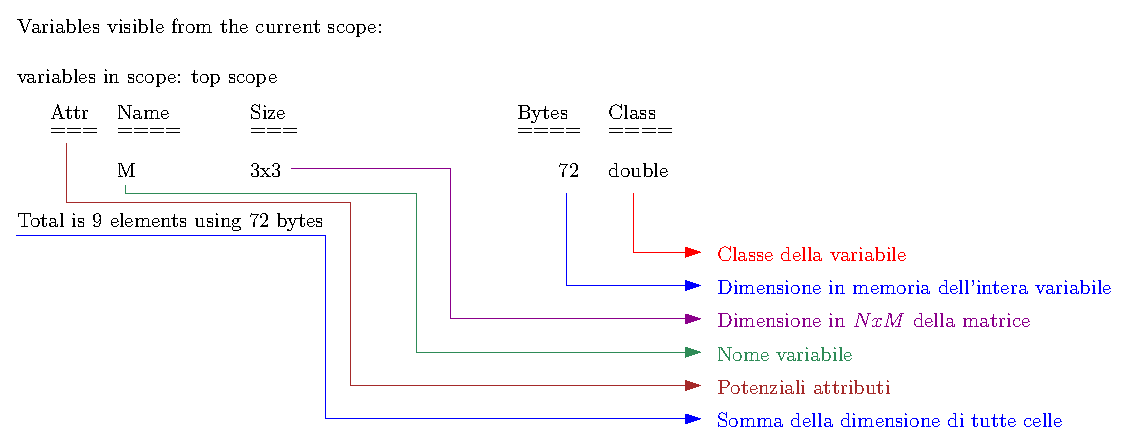
\includegraphics[width=15cm]{img/finiti/whos.eps}
  \caption{descrizione dell'interfaccia di funzione}
  \label{fig:interffun}
\end{figure}
\begin{notab}
  Anche la variabile singola viene vista come una matrice 1x1, da questo si
  denota che come il suo cugino Matlab è un software pensato per elaborare
  prodotti matriciali, infatti, il nome Matlab non sta per \texttt{Mathematic
    lab} ma per \texttt{Matrix Lab}. 
\end{notab}
\subsection{Tipi variabile}
\label{sec:tipivariabile}

\begin{table}[ht]
  \centering
  \begin{tabular}{llll}
    {\bf Nome} & {\bf Descrizione} & {\bf Dimensione} & {\bf Cifre rappresentabili}\\\hline
    \lstinline|double| ({\bf default}) & double-precision array & 8byte & $\pm1.79769x10^{308}$ a $\pm2.22507x10^{-308}$\\\hline
    \lstinline|single| & single-precision array & 4byte & $-2.1475x10^9$ a $2.1475x10^9$\\\hline 
    \lstinline|int8| & Array di interi con segno & 8bit & $-128$ a $127$\\\hline
    \lstinline|int16| & Array di interi con segno & 16bit & $-32768$ a $32767$ \\\hline
    \lstinline|int32| & Array di interi con segno & 32bit & $-2.1475x10^9$ a $2.1475x10^9$\\\hline 
    \lstinline|int64| & Array di interi con segno & 64bit & $-9.2234x10^{18}$ a $9.2234x10^{18}$\\\hline
    \lstinline|uint8| & Array di interi senza segno & 8bit & $255$\\\hline
    \lstinline|uint16| & Array di interi senza segno & 16bit & $65535$ \\\hline
    \lstinline|uint32| & Array di interi senza segno & 32bit & $4.2950x10^9$\\\hline 
    \lstinline|uint64| & Array di interi senza segno & 64bit & $1.8447x10^{19}$\\\hline
  \end{tabular}
  \caption{Tipi variabile}
  \label{tab:tipivariabile}
\end{table}
\begin{oss}
  Questa rapresentazione in memoria vale per la singola cella, quindi bisogna
  moltiplicare il paso per il numero di celle dello stesso tipo. Il programma
  peserà quanto il numero complessivo delle variabili presenti.
\end{oss}

\paragraph{Le stringhe --}
Un altro tipo di variabile però implicita sono le stringhe che il programma può
gestire, nel sequente modo \lstinline|str = "string x"| e la stampa di stringa
viene fatta con un semplice \lstinline|printf(str)|.
\clearpage
\subsubsection{Cosa stampa e cosa no}
Nel linguaggio di Matlab e Octave vengono stampate tutte le associazioni,
funzioni e inizializzazioni che non terminano con il ``{\color{red};}''.

\subsection{Impostazioni e formati}
\label{sec:formImp}
\begin{table}[ht]
  \centering
  \begin{tabular}{lll}
    {\bf Nome} & {\bf Descrizione} & {\bf Visuale}\\\hline
    \lstinline|rat| & Aspetto rateo (invece dei numeri reali rende numeri frazionari) & 1/2\\\hline
    \lstinline|short| & Formato breve a decimale fisso con 4 cifre dopo la virgola. (\textit{default}) & 0.5000\\\hline
    \lstinline|long| & Formato lungo a decimale fisso con 15 cifre dopo la virgola per & 0.500000000000000\\
                     &  i valori doppi e 7 cifre dopo la virgola per i valori singoli. \\\hline
    \lstinline|shortE| & Formato breve in annotazione scientiica con 4 cifre dopo la virgola & 5.0000e-01\\\hline
    \lstinline|longE| & Formato lungo a decimale fisso con 15 cifre dopo la virgola per & 5.000000000000000e-01\\
               & i valori doppi e 7 cifre dopo la virgola per i valori singoli.\\\hline
    \lstinline|shortG| & Formato breve, decimale fisso o notazione scientifica, a seconda & 0.5000\\
               & di quale sia più compatto, con un totale di 5 cifre.\\\hline
    \lstinline|longG| & Formato lungo a decimali fissi o notazione scientifica, qualunque & 0.500000000000000\\
               & sia il più compatto, con un totale di 15 cifre per i valori doppi e\\ & 7 cifre per i valori singoli.\\\hline
    \lstinline|shortEng| & Breve notazione ingegneristica (l'esponente è un
                           multiplo & 500.0000e-003\\
    
               &di 3) con 4 cifre dopo la virgola.\\\hline
    \lstinline|longEng| & Notazione ingegneristica lunga (l'esponente è un multiplo di 3) & 500.000000000000000e-003\\ & con 15 cifre significative.\\\hline
    \lstinline|+|&Formato positivo/negativo con caratteri +, - e vuoti visualizzati & +\\
               & per elementi positivi, negativi e zero.\\\hline
    bank & Formato valuta con 2 cifre dopo la virgola. & 0.50 \\\hline
    hex & Rappresentazione esadecimale di un numero binario & 3fe0000000000000 \\
               & a doppia precisione.\\\hline 
  \end{tabular}
  \caption{Impostazioni e formati}
  \label{tab:form}
\end{table}
\begin{notab}
  È possibile salvare il formato in una variabile con il comando \lstinline|fmt = format("nomeFormato")|
  per poi riutilizzarlo in seguito richiamando \lstinline|format(fmt)|. Altro aspetto esso può cambiare durante lo script quindi è possibile ripotare un dato
  in un formato di stampa e uno in un altro.
\end{notab}
